\documentclass[11pt]{article}
\usepackage{fullpage}
\usepackage{amsmath,amsthm,amssymb,amsfonts,multirow}
\usepackage{mathtools}
\usepackage{graphicx}
\usepackage{xcolor}
\usepackage{float}
%\usepackage{enumerate}
\usepackage[shortlabels, inline]{enumitem}
\usepackage{textcomp}
\usepackage{hyperref}
\usepackage{comment}

\usepackage{listings}
\lstset{language=Python, numbers=left, basicstyle=\ttfamily, keywordstyle=\color{blue}, showstringspaces=false}

\usepackage[style=alphabetic-verb]{biblatex}
% \bibliography{Problems/ref.bib}

\newcommand{\N}{\mathbb{N}}
\newcommand{\Z}{\mathbb{Z}}
\newcommand{\Q}{\mathbb{Q}}
\newcommand{\R}{\mathbb{R}}
\newcommand{\C}{\mathcal{C}}
\newcommand{\K}{\mathbb{K}}
\renewcommand{\div}{\mid}
\newcommand{\ndiv}{\nmid}
\newcommand{\E}{\mathbb{E}}
\newcommand{\I}{\mathbb{I}}
\newcommand{\F}{\mathcal{F}}

\DeclareMathOperator{\id}{Id}
\DeclareMathOperator{\tr}{Tr}
\DeclareMathOperator*{\argmax}{arg\,max}
\DeclareMathOperator{\lcm}{lcm}
\DeclareMathOperator{\spn}{span}
\DeclareMathOperator{\acosh}{acosh}

\DeclarePairedDelimiter{\floor}{\lfloor}{\rfloor}
\DeclarePairedDelimiter{\ceil}{\lceil}{\rceil}
\DeclarePairedDelimiter{\abs}{\lvert}{\rvert}

\newcommand{\subtag}[1]{\tag{\theparentequation#1}}

\renewcommand{\vec}[1]{\mathbf{#1}}

\usepackage{subfiles}
\usepackage{subcaption}
\makeatletter
\newcommand\nocaption{
    \renewcommand\p@subfigure{}
    \renewcommand{\thesubfigure}{\arabic{figure}\alph{subfigure}}
}
\makeatother


\newenvironment{problem}[2][Q]{\begin{trivlist}
\item[\hskip \labelsep {\bfseries #1}{\bfseries #2}]}{\end{trivlist}}

\newenvironment{solution}{%
  \begin{proof}[\textbf{Solution}]$ $\par\nobreak\ignorespaces
}{%
  \end{proof}
}

\theoremstyle{definition}
\newtheorem{definition}{Definition}
\newtheorem{theorem}{Theorem}
\newtheorem{lemma}{Lemma}

\hypersetup{
    colorlinks=true,
    linkcolor=blue,
    filecolor=magenta,      
    urlcolor=cyan,
    pdftitle={Overleaf Example},
    pdfpagemode=FullScreen,
    }


\title{Intro to Computational Mathematics: Section 8}
\date{October 2025}

\begin{document}
\maketitle

\begin{problem}{5.1.2}
    The following table gives life expectancy in the U.S. by year of birth.
    
    \begin{center}
    \begin{tabular}{c|c|c|c|c|c|c}
        \textbf{1980} & \textbf{1985} & \textbf{1990} & \textbf{1995} & \textbf{2000} & \textbf{2005} & \textbf{2010} \\\hline
        73.7 & 74.7 & 75.4 & 75.8 & 77.0 & 77.8 & 78.7
    \end{tabular}
    \end{center}
    
    \begin{enumerate}[(a)]
        \item Defining ``year since 1980'' as the independent variable, follow the method of \href{https://fncbook.com/interpolation/#demo-interpolation-global}{Example 5.1.1} to construct and plot the polynomial interpolant of the data.
        \item Follow the method of \href{https://fncbook.com/interpolation/#demo-interpolation-pwise}{Example 5.1.3} to construct and plot a piecewise cubic interpolant of the data.
        \item Use both methods to estimate the life expectancy for a person born in 2007. Which value is more believable?
    \end{enumerate}
\end{problem}
\begin{solution}
The following code produces the desired polynomial and cubic spline interpolations:

\begin{lstlisting}
import numpy as np
import matplotlib.pyplot as plt
from scipy.interpolate import interp1d

t = [0, 5, 10, 15, 20, 25, 30]
life = [73.7, 74.7, 75.4, 75.8, 77.0, 77.8, 78.7]

plt.scatter(t, life, label='data')
plt.xlabel('Years Since 1980')
plt.ylabel('Life Expectancy')

p = np.poly1d(np.polyfit(t, life, len(t) + 1))

t_ = np.linspace(0, 30, 400)
plt.plot(t_, p(t_), label='Poly Interpolant')

c = interp1d(t, life, kind='cubic')
plt.plot(t_, c(t_), label='Cubic Interpolant')

plt.axvline(2007-1980, color='gray', label='2007')
plt.scatter([2007-1980, 2007-1980], [p(2007-1980), c(2007-1980)], color='gray')

plt.title('Comparison of Interpolation Methods')
plt.legend()
plt.show()

print('Polynomial Approximation (2007): ' + str(p(2007-1980)))
print('Cubic Spline Approximation (2007): ' + str(c(2007-1980)))
\end{lstlisting}
Output:
\begin{center}
    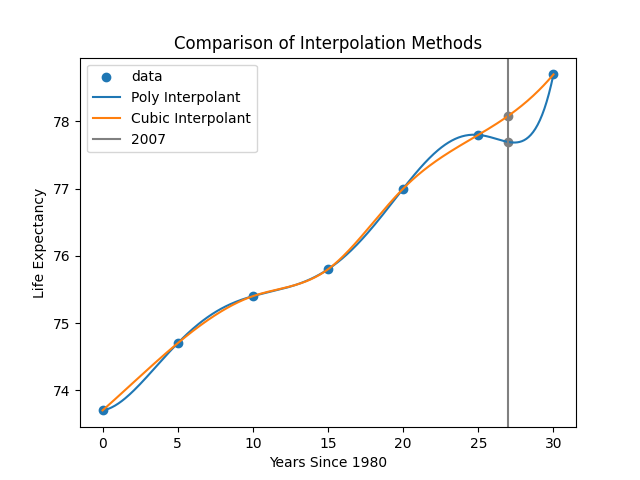
\includegraphics[width=0.8\textwidth]{5.1.2_fig.png}
\end{center}
\begin{verbatim}
    Polynomial Approximation (2007): 77.69430093045608
    Cubic Spline Approximation (2007): 78.08420000000001
\end{verbatim}

We should trust the cubic interpolant more than the polynomial interpolant here.
\end{solution}



\begin{problem}{5.1.3}
    The following two vectors define a flying saucer shape.
    $$x = [ 0, 0.51, 0.96, 1.06, 1.29, 1.55, 1.73, 2.13, 2.61, 2.19, 1.76, 1.56, 1.25, 1.04, 0.58, 0 ]$$
    $$y = [ 0, 0.16, 0.16, 0.43, 0.62, 0.48, 0.19, 0.18, 0, -0.12, -0.12, -0.29, -0.30, -0.15, -0.16, 0 ]$$
    We can regard both $x$ and $y$ as functions of a parameter $s$, with the points being values given at $s = 0, 1, \ldots, 15$.
    \begin{enumerate}[(a)]
        \item Follow the method of \href{https://fncbook.com/interpolation/#demo-interpolation-pwise}{Example 5.1.3} to make cubic spline interpolants of each coordinate as functions of $s$, and make a picture of the flying saucer.
        \item (\textit{Julia only}) One drawback of the result in part (a) is the noticeable corner at the left side, which corresponds to $s = 0$ from above and $s = 15$ from below. There is a periodic variation on cubic spline interpolation that you can invoke by adding the keyword {\color{red}\texttt{periodic=true}} to the {\color{red}\texttt{Spline1D}} call. Use this to re-plot the flying saucer.
    \end{enumerate}
\end{problem}
\begin{solution}
\begin{lstlisting}
import numpy as np
import matplotlib.pyplot as plt
from scipy.interpolate import interp1d

x = [0, 0.51, 0.96, 1.06, 1.29, 1.55, 1.73, 2.13, 2.61, 2.19, 1.76, 1.56, 1.25, 1.04, 0.58, 0]
y = [0, 0.16, 0.16, 0.43, 0.62, 0.48, 0.19, 0.18, 0, -0.12, -0.12, -0.29, -0.30, -0.15, -0.16, 0]

s = [i for i in range(len(x))]

x_ = interp1d(s, x, kind='cubic')
y_ = interp1d(s, y, kind='cubic')

s_ = np.linspace(0, 15, 400)
plt.scatter(x, y, label='data')
plt.plot(x_(s_), y_(s_), label='Spline Approx')
plt.title('Drawing A UFO With Splines')
plt.legend()
plt.show()
\end{lstlisting}
Output:
\begin{center}
    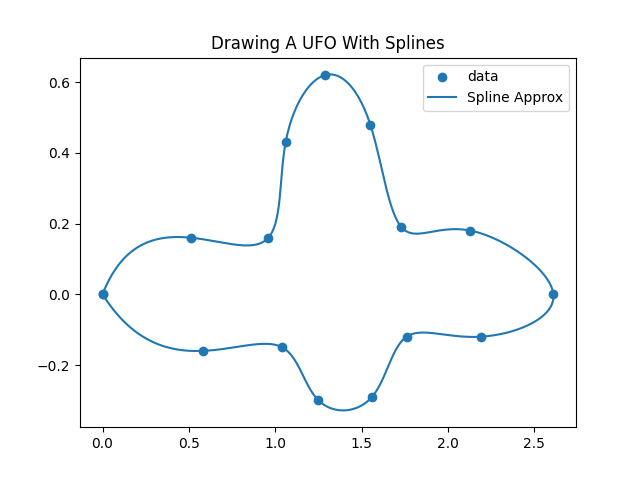
\includegraphics[width=0.8\textwidth]{5.1.3_fig.png}
\end{center}
\end{solution}



\begin{problem}{5.1.4}
    Define $$q(s) = a\frac{s(s-1)}{2} - b(s-1)(s+1) + c\frac{s(s+1)}{2}.$$
    \begin{enumerate}[(a)]
        \item Show that $q$ is a polynomial interpolant of the points $(-1, a), (0, b), (1, c)$.
        \item Find a change of variable $s = Ax + B$ so that the values $s = -1, 0, 1$ correspond to $x = x_0 - h, x_0, x_0 + h$.
        \item Find a quadratic polynomial interpolant $\tilde{q}(x) = q(s)$ for the points $(x_0 - h, a), (x_0, b), (x_0 + h, c)$.
    \end{enumerate}
\end{problem}
\begin{solution}
\begin{enumerate}[(a)]
    \item
        \begin{align*}
            q(-1) &= a\frac{-1(-1-1)}{2} - b(-1-1)(-1+1) + c\frac{-1(-1+1)}{2} \\
            &= a\frac{-1(-2)}{2} - b(-2)(0) + c\frac{-1(0)}{2} \\
            &= a \\
            q(0) &= a\frac{0(0-1)}{2} - b(0-1)(0+1) + c\frac{0(0+1)}{2} \\
            &= b \\
            q(1) &= a\frac{1(1-1)}{2} - b(1-1)(1+1) + c\frac{1(1+1)}{2} \\
            &= a\frac{1(0)}{2} - b(0)(2) + c\frac{1(2)}{2} \\
            &= c
        \end{align*}
    \item We want $A(x_0 + h) + B = 1$ and $A(x_0) + B = 0$. This implies that $Ah = 1$ and that $A = 1/h$. Plugging in to the second equation, we get $B = -x_0/h$.
    \item Substituting in $s = \frac{x}{h} - \frac{x_0}{h}$ we get:
        \begin{align*}
            \tilde{q}(x) &= a\frac{(\frac{x}{h} - \frac{x_0}{h})(\frac{x}{h} - \frac{x_0}{h} - 1)}{2} - b(\frac{x}{h} - \frac{x_0}{h} - 1)(\frac{x}{h} - \frac{x_0}{h} + 1) + c\frac{(\frac{x}{h} - \frac{x_0}{h})(\frac{x}{h} - \frac{x_0}{h} + 1)}{2} \\
            &= \frac{a}{2h^2}(x - x_0)(x - x_0 - h) - \frac{b}{h^2}(x - x_0 - h)(x - x_0 + h) + \frac{c}{h^2}(x - x_0)(x - x_0 + h) \\
            &= \frac{a}{2h^2}(x - x_0)(x - (x_0 + h)) - \frac{b}{h^2}(x - (x_0 + h))(x - (x_0 - h)) + \frac{c}{h^2}(x - x_0)(x - (x_0 - h)) \\
        \end{align*}
\end{enumerate}
\end{solution}



\begin{problem}{5.1.5}
    (continuation) Use the result of the previous exercise and \href{https://fncbook.com/interpolation/#theorem-interp-conditioning}{Thereom 5.1.1} to derive bounds on the condition number of the quadratic polynomial interpolation at the nodes $x_0 - h, x_0, x_0 + h$.
\end{problem}
\begin{solution}
    Define $\phi_{-1}, \phi_0, \phi_1$ as the cardinal functions that interpolate with $\phi_i(x_0 - ih) = 1, \phi_i(x_0 - jh) = 0$ for $j \neq i$ ($j \in \{-1, 0, 1\}$).

    We then can write the previous polynomial interpolation as:
    \begin{align*}
        \tilde{q}(x) &= \frac{a}{2h^2}(x - x_0)(x - (x_0 + h)) - \frac{b}{h^2}(x - (x_0 + h))(x - (x_0 - h)) + \frac{c}{h^2}(x - x_0)(x - (x_0 - h)) \\
        &= a \phi_{-1}(x) + b \phi_0(x) + c \phi_1(x)
    \end{align*}

    Theorem 5.1.1 tells us that $\kappa_{\tilde{q}}(x) \leq \sum_{k = -1}^{1}\|\phi_k\|_\infty$.
    In the range $[x_0 - h, x_0 + h]$, we have: $\|\phi_i\|_\infty = 1$ for each $i$, so $\kappa_{\tilde{q}}(x) \leq 3$.
    \end{solution}
    
\end{document}
